\thispagestyle{sectioned}
\chapter{AppearWOW: A Wave Gadget}
\label{subsec:video_intro}
%\addcontentsline{toc}{chapter}{\numberline{Video Conference Gadget}}
Design Guidelines report of the P2P value project claims that ``The platform should therefore include tools for collaboration, including key features, such as: Synchronous communication'', among these synchronous tools they mention ``Video and voice communication'' \cite{ref:p2pvalue}.\\[.2cm]
Wave is meant for text communication. Text has the advantage that it can be stored easily, searched later and edited simultaneously, but lacks the naturallity of human-to-human interaction. To get as close as possible to it we need voice and video. Then collaborating on text can be made more efficiently. This gadget makes it possible to \textbf{speak to up to 16 other users and see them}.
\section{State of the Art}
\label{subsec:video_soa}
There is no alternative to video or audio communication integrated on Wave. There is other alternatives though outside of it, some of them shown in Figure \ref{fig:skype_hangouts}.
\begin{figure}[h]
  \center
    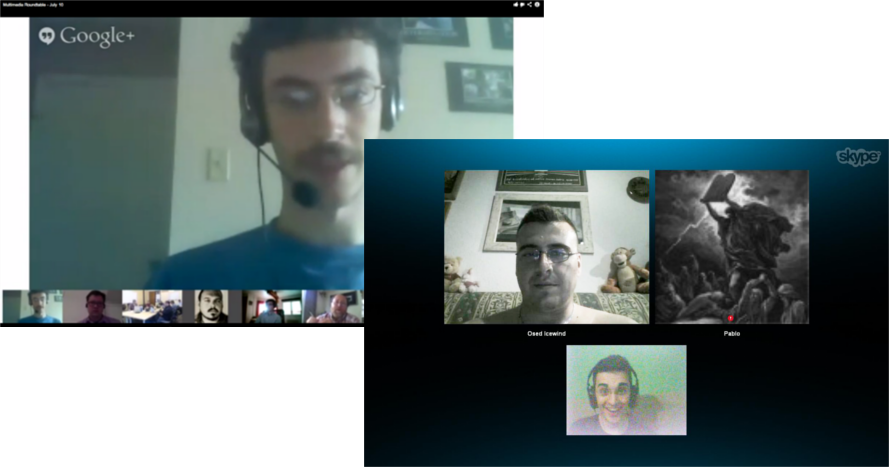
\includegraphics[keepaspectratio, scale=0.43]{Media/Captures/Soa/skype_hangouts.png}
  \caption{Hangouts and Skype}
  \label{fig:skype_hangouts}
\end{figure}
They focus on video, even hiding text communication to leave more room to the video. AppearWOW can be mixed with text above and below, leaving the video communication as an addition and not the main point. Both video communication tools shown (Google's Hangouts and Microsoft's Skype) require you to have a specific user account to use their services, while this gadget lets you join the \textbf{video communication from within Wave}, but also from an external link without giving any kind of personal information.

\section{Results}
To make this gadget it has been essential the use of a pre-existing service called \textbf{appear.in} \cite{ref:appearin}. They provide the whole video and audio communication based on WebRTC \cite{ref:webrtc}, and also facilitate an easy way to use their service in an external website. It is a JavaScript component that can be put inside an iframe, and it will take care of almost everything. Figure \ref{fig:video_gadget} shows the final result of this integration.
\begin{figure}[h]
  \center
    
\includegraphics[keepaspectratio, scale=0.8]{Media/Captures/Extensions/VideoGadget/RoomSelection.png}
  \caption{Room Selection Screen}
  \label{fig:video_gadget_room}
\end{figure}
When a user inserts the gadget, he will be prompted with the room selection screen shown in Figure \ref{fig:video_gadget_room}, letting him choose the identifier of the room people will meet in. The same room can be visited from different waves, and also directly from appear.in, as room names can not be duplicated.
\begin{figure}[h]
  \center
    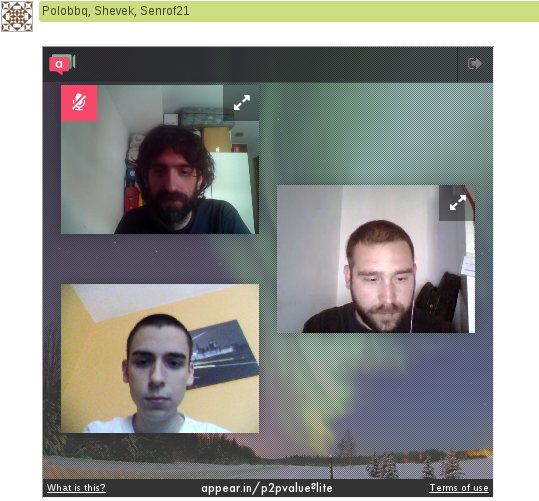
\includegraphics[keepaspectratio, scale=0.45]{Media/Captures/Extensions/VideoGadget.png}
  \caption{Video Conference Gadget}
  \label{fig:video_gadget}
\end{figure}
It was shown in Figure \ref{fig:gadget_classes} the basic structure of a gadget. The composite is represented by the VideoGadgetMainPanel, the Messages are the class VideoGadgetMessages, and the GinModule is realised by VideoGadgetGinModule. Outside from that, the structure is relatively simple.\\[.2cm]
As appear.in is a JavaScript service, multiple calls to \textbf{native JavaScript} have been made inside this gadget.
The service appear.in uses the name of the room as a unique identifier, so the gadget asks the user for a name before entering the room. The gadget also makes use of appear.in's \verb|?lite| feature, that simplifies the user interface, leaving more space for the images of the video. The \textbf{camera is accessed through the browser}, so no additional software has to be installed.\\[.2cm]
The Wave state in this gadget is really simple, the only thing stored in it is the name of the room to enter it directly if it has already been set.\\[.2cm]
\begin{figure}[h]
  \center
    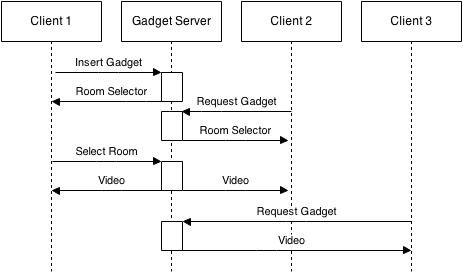
\includegraphics[keepaspectratio, scale=0.6]{Media/Diagrams/Gadget/VideoSequence.png}
  \caption{UML Sequence Diagram, AppearWOW}
  \label{fig:video_gadget_sequence}
\end{figure}
Figure \ref{fig:video_gadget_sequence} shows how the gadget reacts to requests. Once the gadget is inserted, the room selection screen will be shown, allowing any participant to select the name of the room the participants will meet in. When a room is selected, the participants automatically enter the room. If another participant joins the wave once the room has been selected, he will be served the video conference directly.
\section{Conclusions and Future Work}
This Wave extension is a Gadget which allows all the participants who are in the wave to join a video conference among them.\\[.2cm]
The fact that this extension is completely \textbf{dependant on an external closed-source service} is a big limitation. The service could stop working at any time, technical improvements on video or audio communication can not be made, limitations like the maximum of 16 online users can not be avoided, the way to use it could change making it necessary to update the gadget, and other changes may arise.\\[.2cm]
To solve all of these problems, an open source alternative for the video and audio communication should be used, or it should be developed from scratch.
\newpage
